\section{Riktantenner för kortvåg}

\subsection{Riktbar dipol-antenn}
\index{riktbar dipolantenn}
\index{antenn!riktbar dipol-}

\begin{figure}
  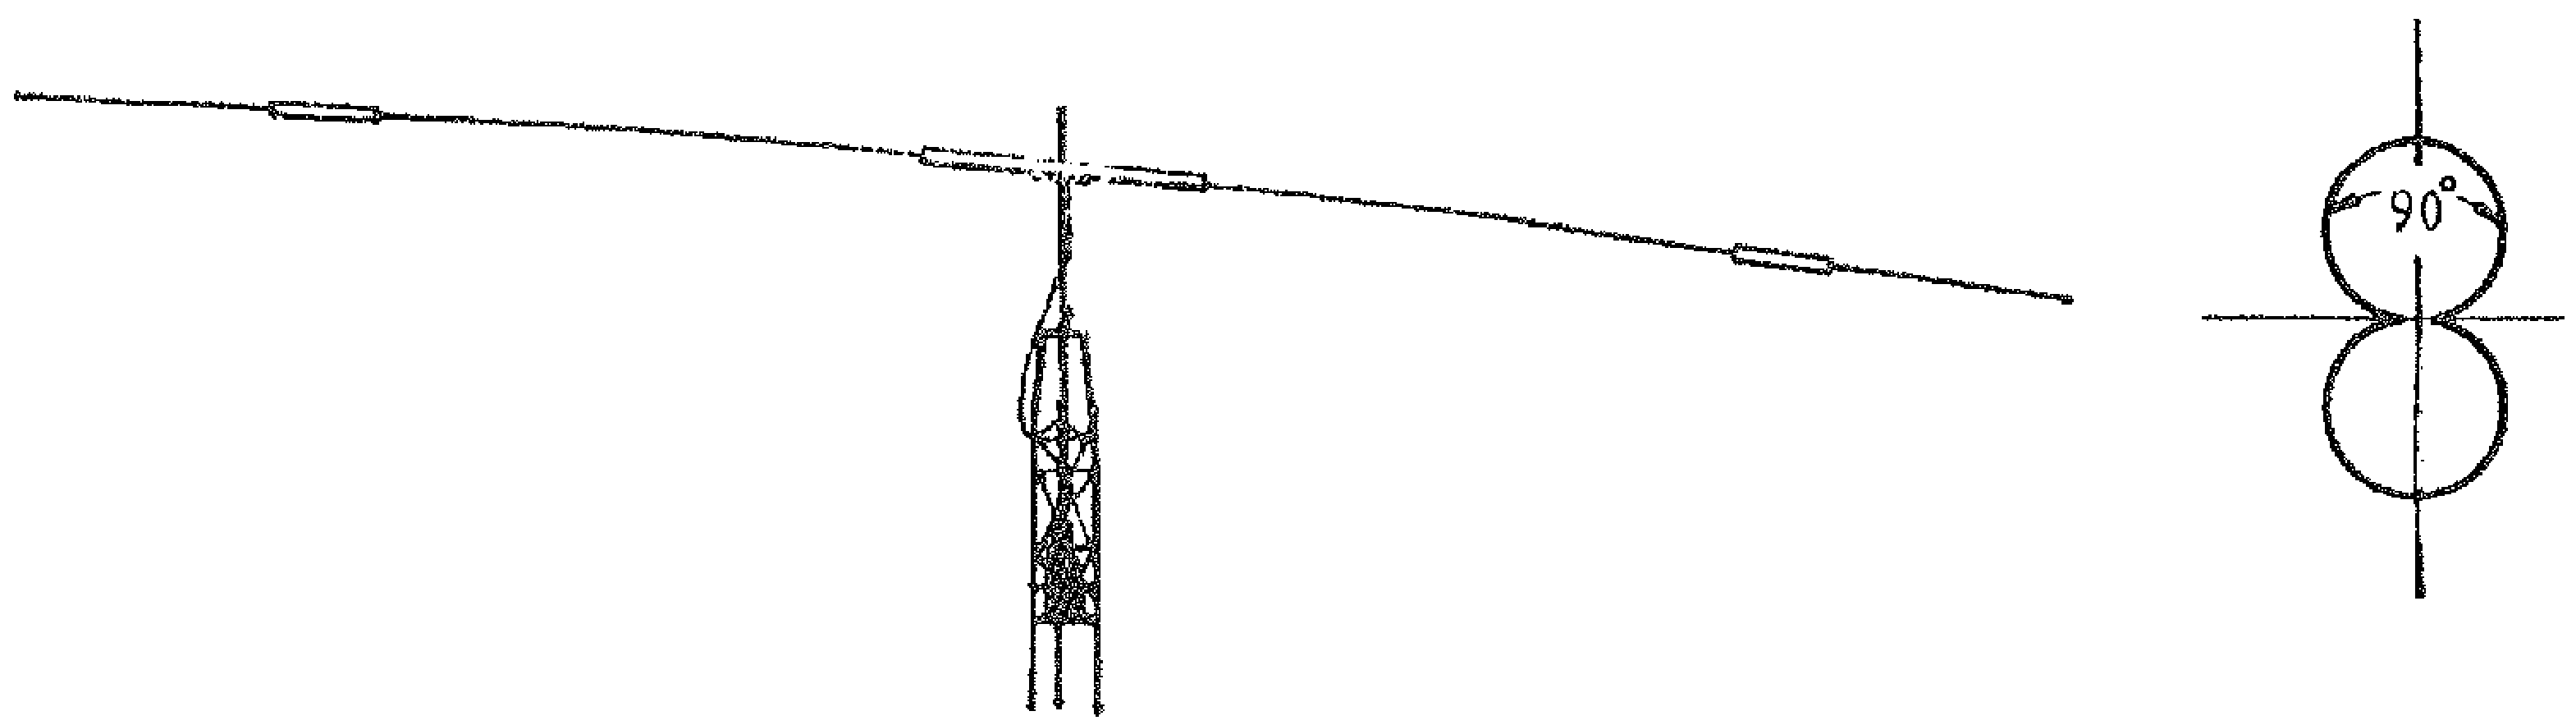
\includegraphics[width=\textwidth]{images/cropped_pdfs/bild_2_6-17.pdf}
  \caption{Riktbar dipol-antenn}
  \label{fig:bildII6-17}
\end{figure}

En dipolantenn av måttlig mekanisk storlek kan göras vridbar så att
utstrålningen kan riktas, så som illustreras i bild \ref{fig:bildII6-17}.
Men eftersom en ensam dipol strålar i många riktningar, låt vara mest vinkelrätt
ut från antennen, så kan energin i de flesta riktningarna ses som ''förlorad''.

När ett passivt antennelement -- en reflektor -- placeras bakom det aktiva
elementet kan emellertid bakåtstrålningen delvis vändas framåt och man får i
stället en viss riktverkan.
För att det ska fungera ska de båda elementen ha ett visst inbördes förhållande
mellan elementens längd och avståndet mellan elementen.


\subsection{Yagiantenner}
\textbf{
HAREC a.\ref{HAREC.a.6.1.5}\label{myHAREC.a.6.1.5}
}
\index{yagiantenn}
\index{antenn!yagi-}
\index{monobandbeam}
\index{antenn!monobandbeam}
\index{multibandbeam}
\index{antenn!multibandbeam}

\begin{figure}
  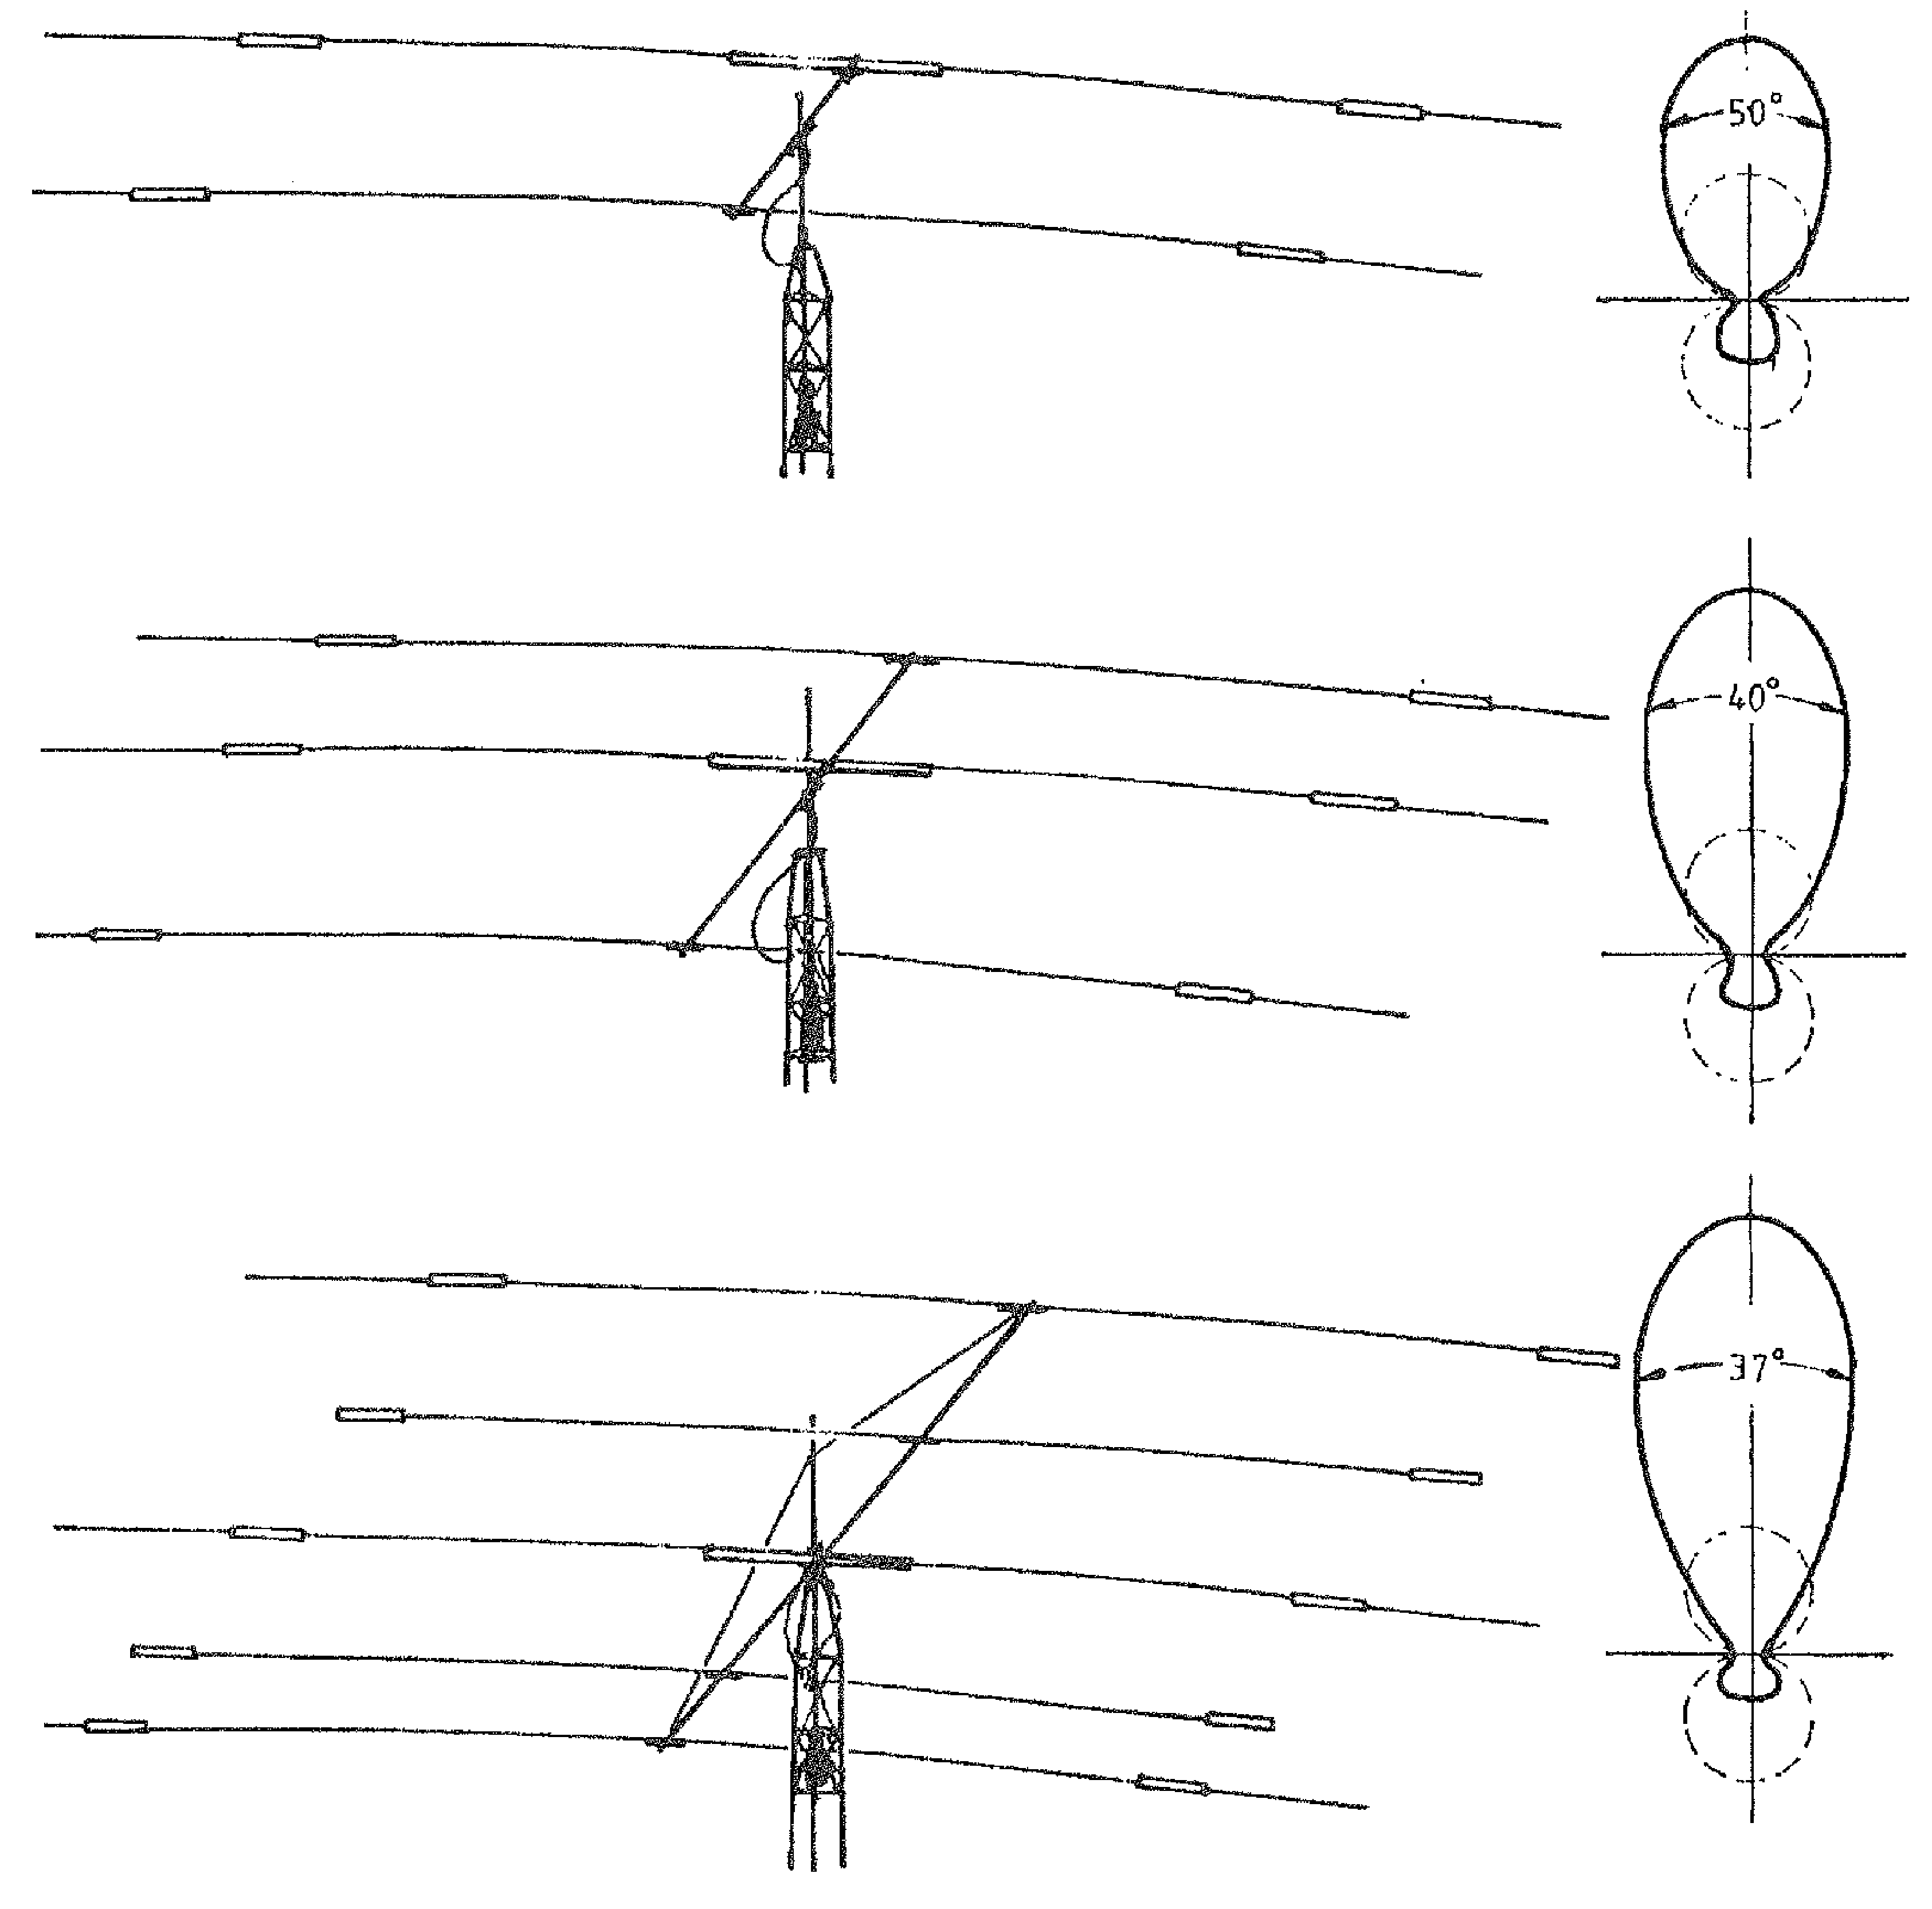
\includegraphics[width=\textwidth]{images/cropped_pdfs/bild_2_6-18.pdf}
  \caption{flerbands yagiantenner}
  \label{fig:bildII6-18}
\end{figure}

Med ytterligare passiva antennelement -- s.k. direktorer -- framför det
aktiva elementet, blir riktverkan ännu bättre.
Reflektorn är alltid elektriskt längre än det aktiva elementet och direktorerna
är alltid elektriskt kortare.
Direktorernas längd blir kortare på längre avstånd från det drivna elementet.
Läs mer om riktantenner i kapitel \ref{riktantenn}.

En sådan antenn är Yagi-Uda-antennen, döpt efter sina japanska upphovsmän.
Den kallas oftast enbart för \emph{yagiantenn}.
Den är ursprungligen avsedd för ett enda frekvensband, en s.k.
\emph{monobandbeam}.

Om alla element förses med lämpliga spärrkretsar, med W3DZZ-antennen som
förebild, fås en riktantenn som är användbar på flera frekvensband, en s.k.
\emph{multibandbeam}.
De vanligaste antennerna för flera band har två till tre element och är
konstruerade för frekvensbanden 10~m, 15~m och 20~m.
Bild \ref{fig:bildII6-18} visar flerbands yagiantenner med 2, 3 respektive 5
element samt deras strålningsdiagram i horisontalplanet.
Matningen sker oftast med en koaxialkabel med den karakteristiska impedans 50~\(\Omega\).
Eftersom matningsimpedansen för själva riktantenn nästan aldrig är
50~\(\Omega\), så behövs oftast en impedansanpassning mellan antenn och kabel.

\subsection{Cubical Quad-antenner}
\index{cubical quadantenn}
\index{quadantenn}

\begin{figure}
  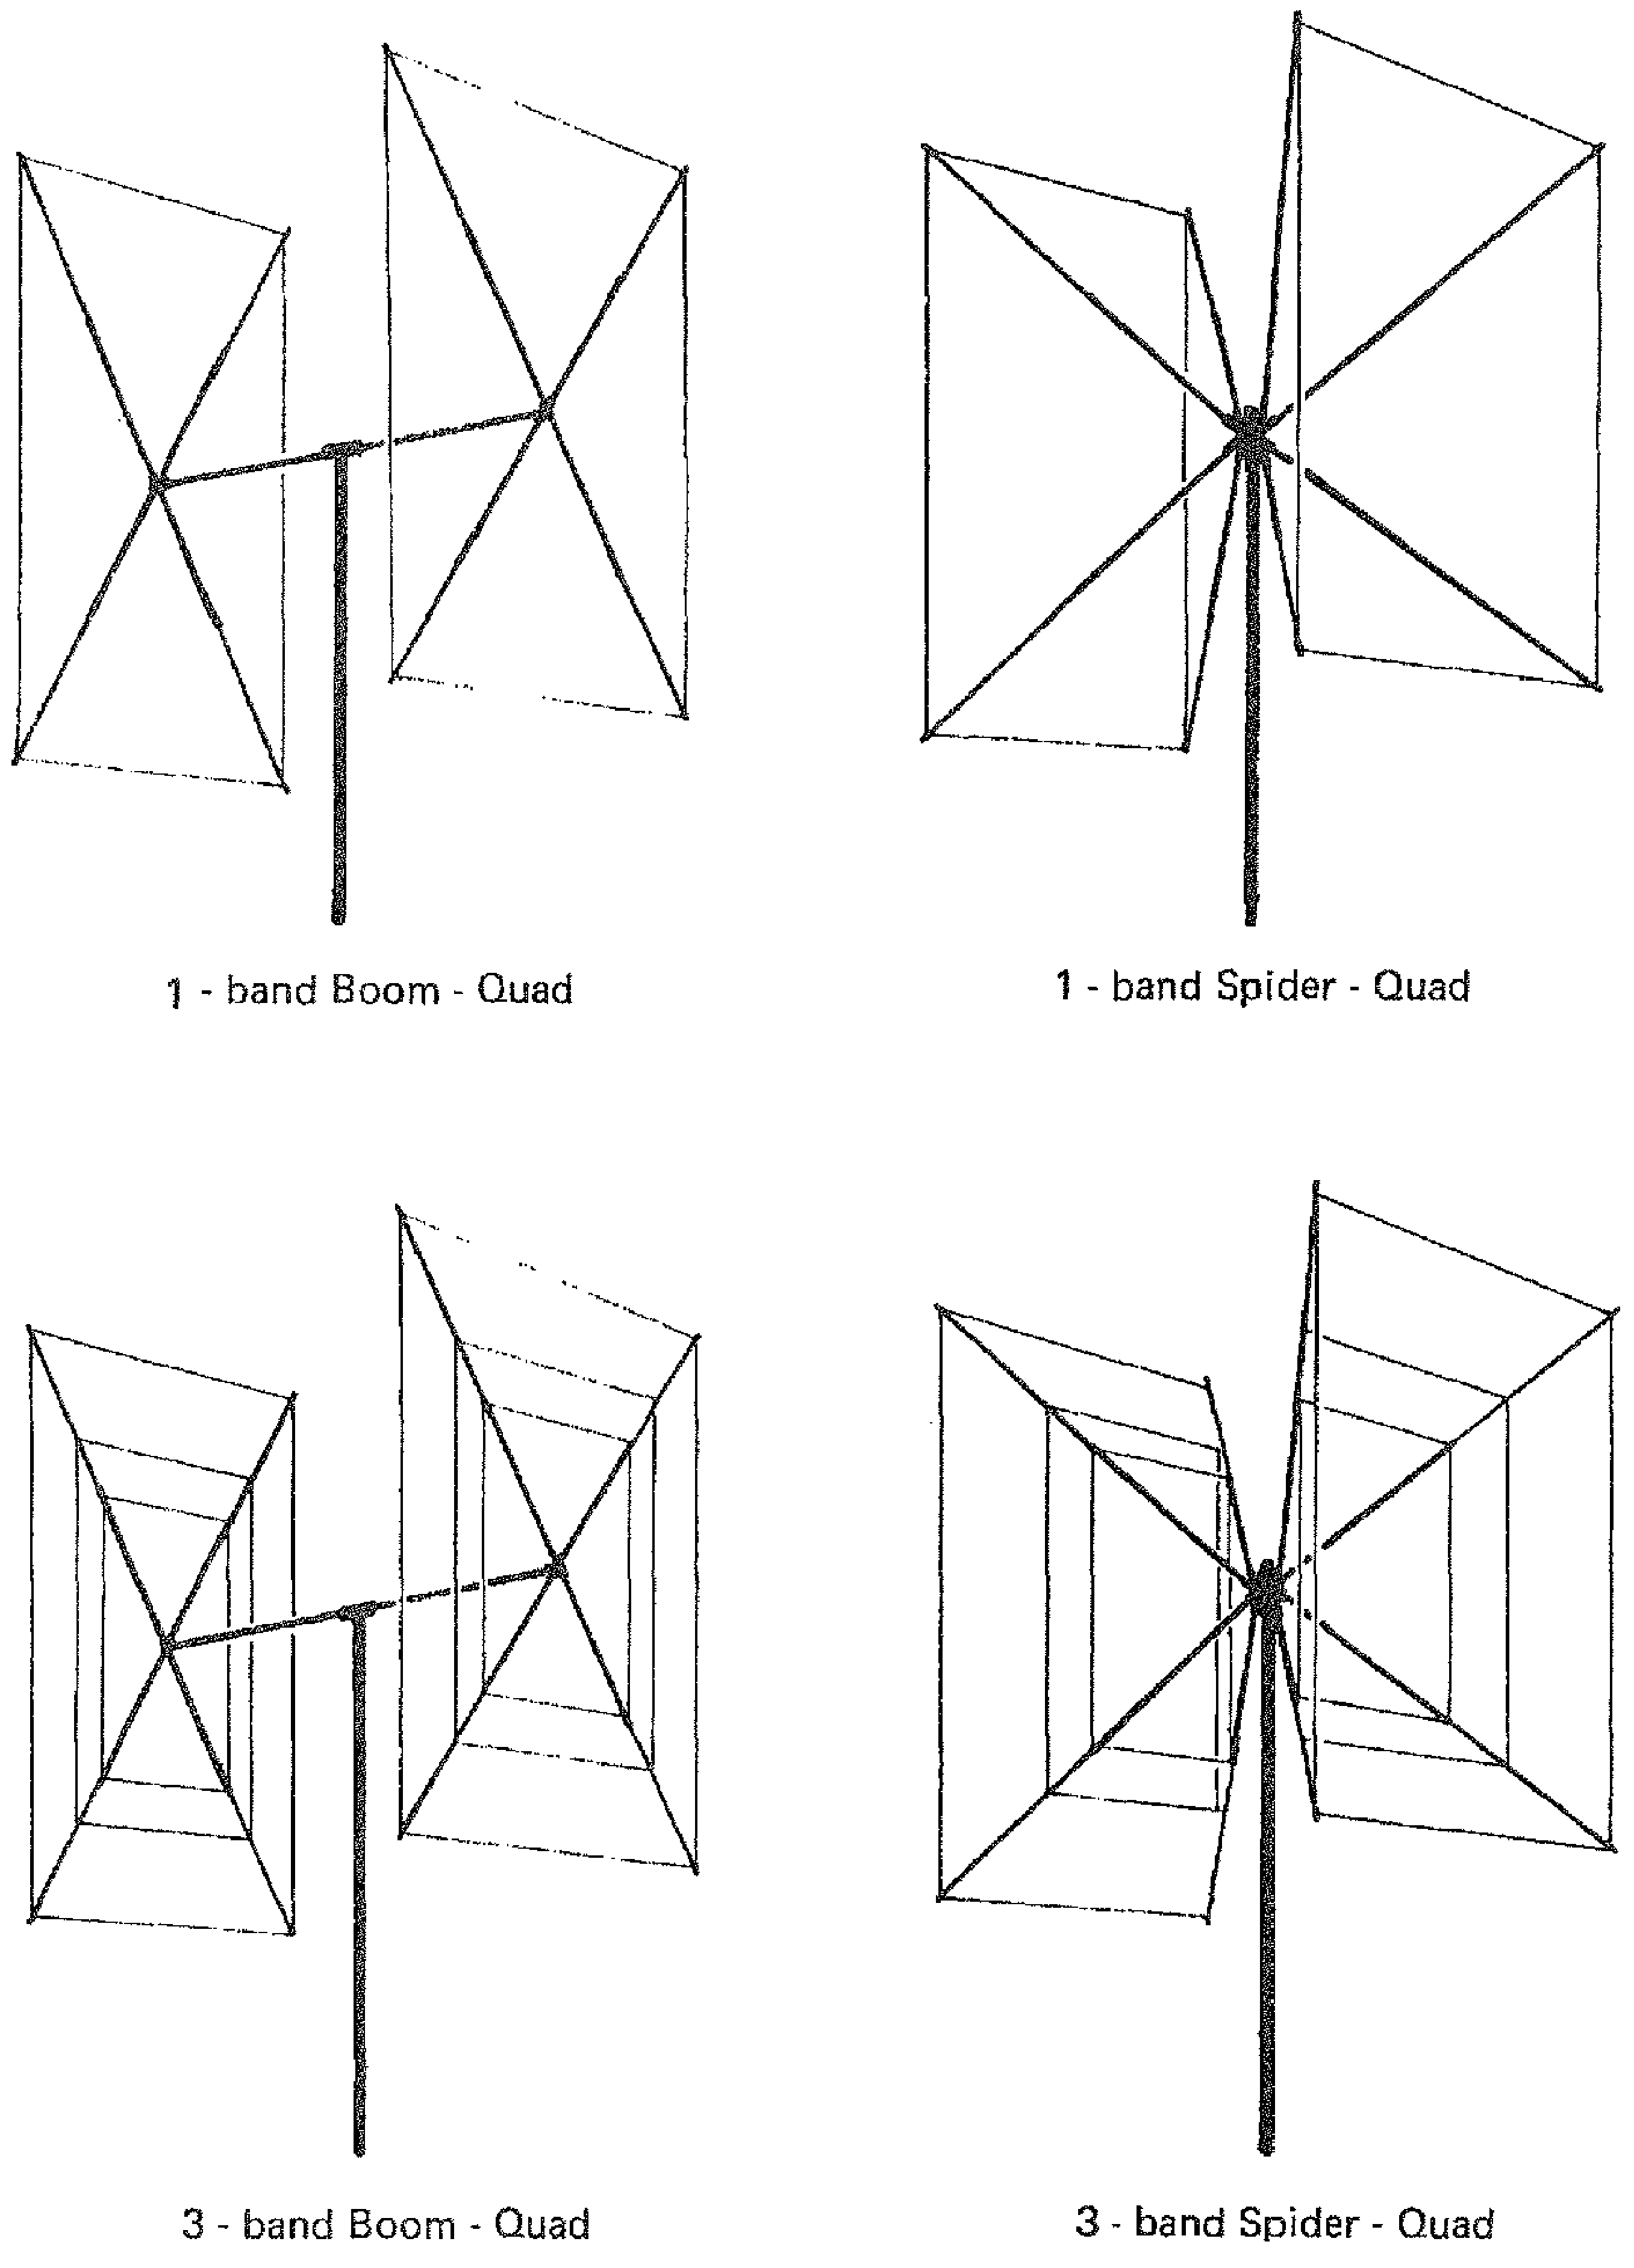
\includegraphics[width=\textwidth]{images/cropped_pdfs/bild_2_6-19.pdf}
  \caption{Cubical Quad-antenner}
  \label{fig:bildII6-19}
\end{figure}

Bild \ref{fig:bildII6-19} visar en \emph{cubical quad-antennen} som är en
kvadratisk helvågsstrålare med en sidlängd av \(\lambda/4\), det vill säga
totalt \(1\lambda\).

En 2-elements quad-antenn består av en strålare och en reflektor på
ett inbördes avstånd av 0,15--0,2 \(\lambda\).
Det finns även 3 och 4-elements quad-konstruktioner med beaktansvärda
dimensioner.
Antennen görs lämpligen vridbar och bör monteras åtminstone \(3/4 \lambda\)
över mark.

Matningen sker oftast med en koaxialkabel och beroende på elementavståndet
varierar matningsimpedansen mellan 50 till 70~\(\Omega\).
Beroende på hur matningspunkten placeras är det möjligt att välja mellan
horisontell eller vertikal polarisering.

Det finns två utföranden av quad-antenner, det ena med en bärande bom
med spridare för att bära upp antennelementen och det andra med bara
spridare från ett centralt fäste, den s.k. spider quad (spindel).

Quad-antenner byggs vanligen för 10-, 15- och 20~m-banden.
Spiderprincipen är att föredra vid utförande för flera band, eftersom ett
optimalt elementavstånd kan väljas för varje band utan att antalet spridare
behöver ökas.

Genom den flacka strålningsvinkeln är quad-antennen en utmärkt DX-antenn.
En två-elements quad anses kunna ge ett resultat som en 3-elements yagiantenn.

För kortvågsbruk finns många antenntyper, såsom longwire-, zepp-,
windom-, romb-, delta loop-, quad loop-antenner etc. För mer
information hänvisas till antennlitteratur.
